% Provenance (never printed): cycle 2 "Questionner l'espace et le temps"
% (oceans, seas, continents on the globe) and "Questionner le monde de la
% matiere" (states of water in natural phenomena); see sources/book1/PROVENANCE.md.
% Book 1, grade 2, chapter 1.
\chapter{A água na Terra}\label{ch:g2:water-on-earth}

No dia 7 de dezembro de 1972, três astronautas a caminho da Lua viraram a
câmera para trás, em direção à Terra. A foto que tiraram virou uma das
imagens mais famosas de todos os tempos. Observe-a. Dá para ver nuvens
brancas, um pouco de terra marrom e amarela, o gelo branco embaixo --- e
azul, azul por toda parte. Vista do espaço, a nossa Terra é um planeta azul.

\begin{omfigure}
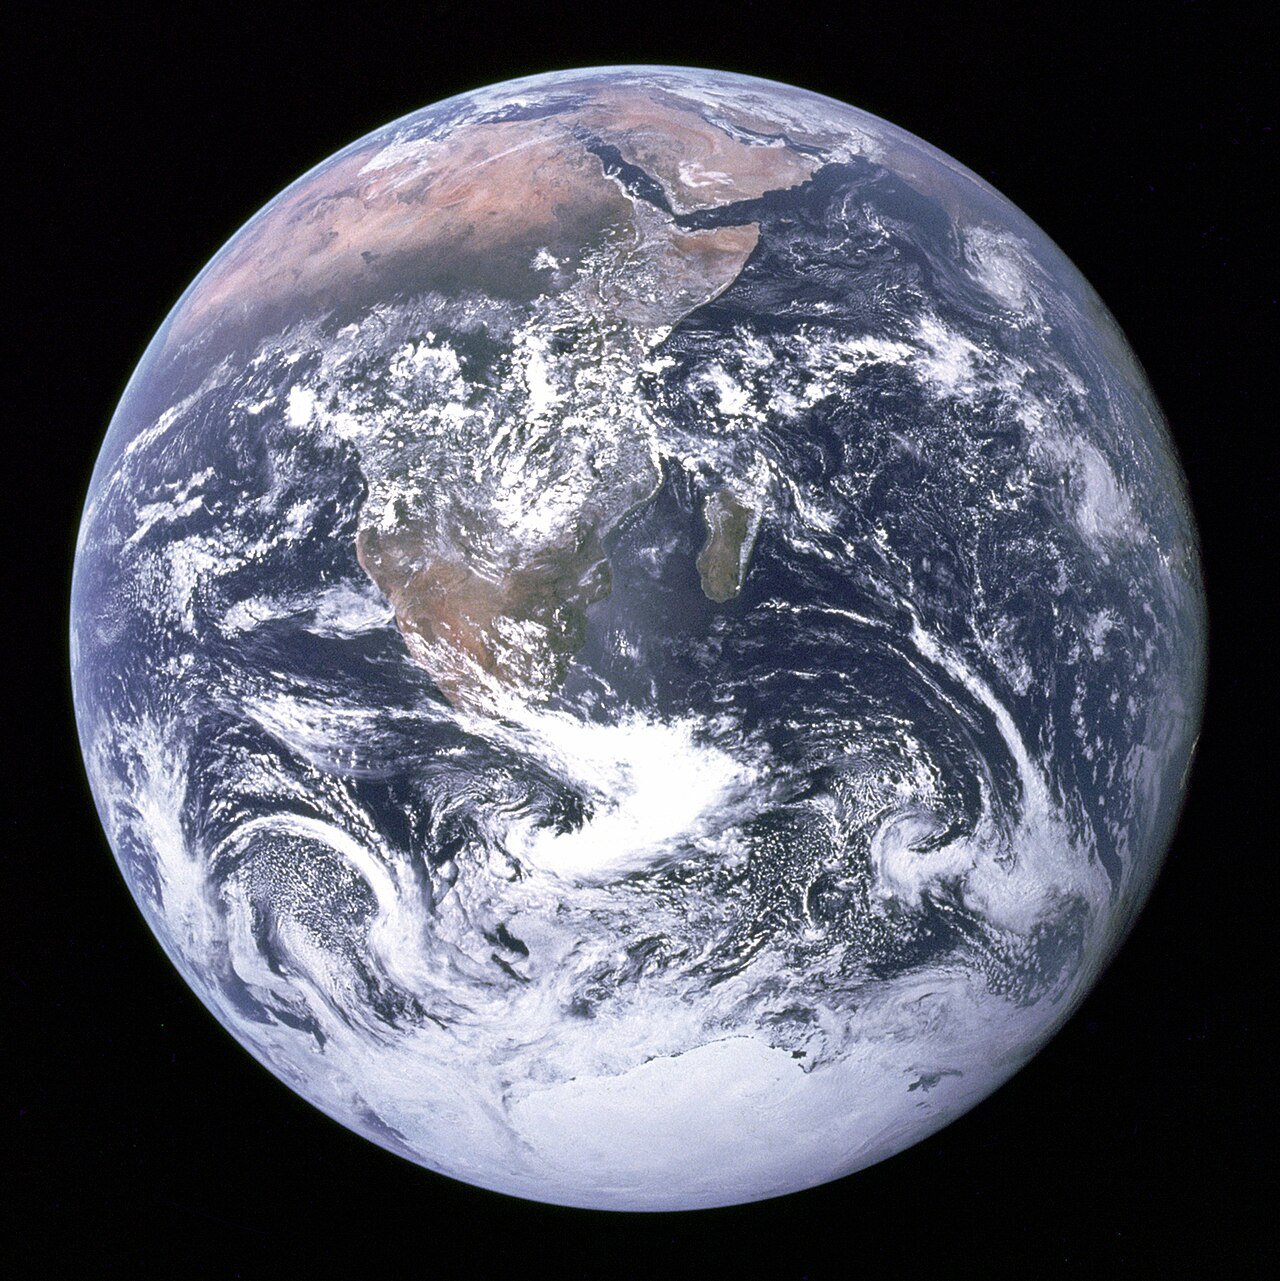
\includegraphics[width=0.5\linewidth]{images/book1/g2-nasa-blue-marble.jpg}

{\small A Terra fotografada pela tripulação da Apollo~17, em 7~de dezembro de 1972.
Vemos a África, a Arábia no alto e o gelo da Antártida embaixo.
Foto: NASA (domínio público).}
\end{omfigure}

\begin{recall}
A água pode ser sólida (gelo), líquida, ou um gás que não conseguimos ver
(o vapor de água). A água líquida deixada ao sol vira vapor aos poucos: ela
evapora. Quando o vapor esfria, ele volta a formar gotinhas: ele se
condensa. Você já viu essas mudanças nos livros de física. Numa \omterm{def:g1:landscapes-around-us:landscape}{paisagem},
a água corre nos \omterm{def:g1:landscapes-around-us:water}{rios} e fica parada nos \omterm{def:g1:landscapes-around-us:water}{lagos} (\cref{ch:g1:landscapes-around-us}).
\end{recall}

\section{O planeta azul}

A maior parte da Terra é coberta de água. Imagine toda a superfície da
Terra cortada em 100 quadrados iguais. Se pintarmos de azul cada quadrado
coberto pelo \omterm{def:g2:water-on-earth:ocean}{mar}, vamos pintar 71 quadrados. Só 29 quadrados são de terra.

\begin{omfigure}
\begin{tikzpicture}
  \begin{axis}[hide axis, width=7.2cm, height=7.2cm, xmin=-0.5, xmax=9.5,
      ymin=-0.5, ymax=9.5, axis equal image, scale only axis,
      clip=false]
    \addplot[scatter, only marks, mark=square*, mark size=9.2pt,
      scatter/classes={0={fill=green!45!omLithAlluv, draw=black!40},
                       1={fill=omSea!80!blue, draw=black!40}},
      point meta=explicit symbolic]
      table[x=col, y=row, meta=blue] {figdata/out/grade-2-ocean_fraction-grid.dat};
  \end{axis}
\end{tikzpicture}

{\small Se a superfície da Terra fosse cortada em 100 quadrados iguais, 71
seriam de \omterm{def:g2:water-on-earth:ocean}{mar} (azul) e 29 de terra (verde). Calculado a partir de um mapa
do relevo de toda a Terra (NOAA ETOPO1).}
\label{fig:g2:water-on-earth:grid}
\end{omfigure}
% ledger: data:etopo1, wss:ocean-cover (71 % computed in figdata/grade-2/ocean_fraction.py)

As grandes extensões de \omterm{def:g2:water-on-earth:salt-fresh}{água salgada} que cobrem a maior parte da Terra têm nomes.

\begin{definition}[Oceano e mar]\label{def:g2:water-on-earth:ocean}
Um \emph{oceano}\index{oceano} é uma das extensões enormes de \omterm{def:g2:water-on-earth:salt-fresh}{água salgada}
que cobrem a maior parte da Terra e ficam entre os continentes. Um
\emph{mar}\index{mar} é uma extensão menor de \omterm{def:g2:water-on-earth:salt-fresh}{água salgada}, em geral na
beira de um oceano e em parte cercada de terra.
\end{definition}

Todos os \omterm{def:g2:water-on-earth:ocean}{oceanos} estão ligados uns aos outros: um barco poderia navegar de
qualquer \omterm{def:g2:water-on-earth:ocean}{oceano} para qualquer outro sem atravessar terra firme. Os nomes
deles, e onde ficam num globo, estão no \cref{ch:g3:continents-and-oceans}.

\begin{omfigure}
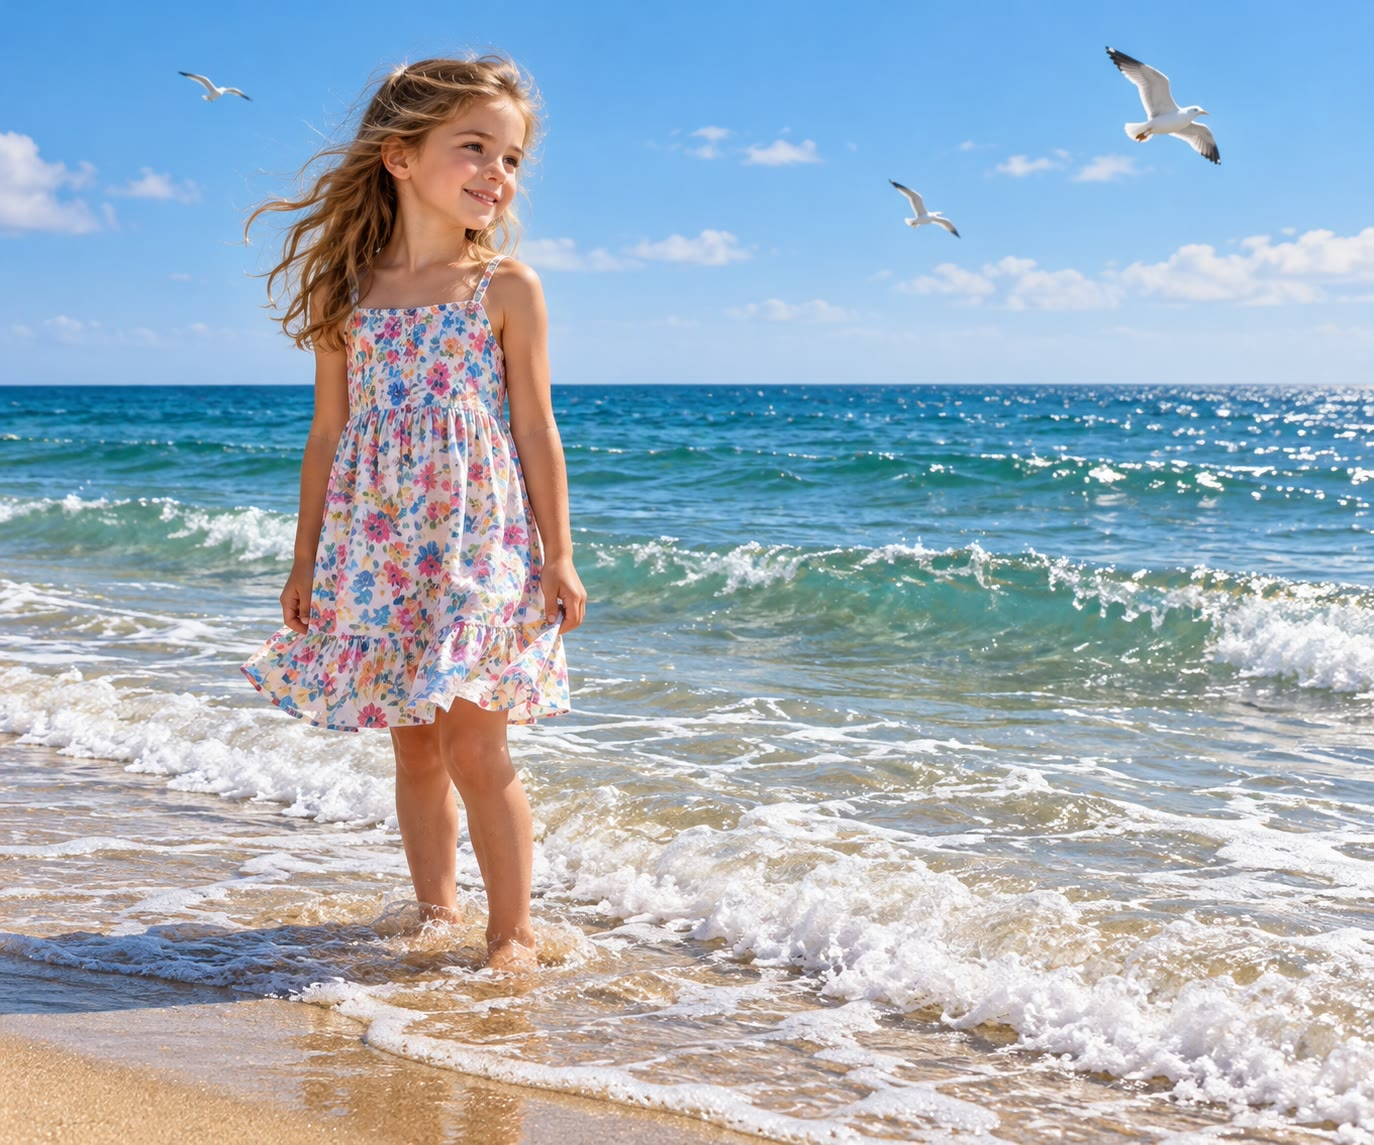
\includegraphics[width=0.62\linewidth]{images/book1/ai/g2-beach-sea.jpg}

{\small Na beira do \omterm{def:g2:water-on-earth:ocean}{mar}. A água continua, muito mais longe do que os olhos
conseguem ver.}
\end{omfigure}

\section{Água salgada e água doce}

Se você já engoliu um gole de água do \omterm{def:g2:water-on-earth:ocean}{mar} enquanto nadava, você sabe: ela
tem um gosto bem salgado. A água dos \omterm{def:g1:landscapes-around-us:water}{rios} e dos \omterm{def:g1:landscapes-around-us:water}{lagos}, não.

\begin{definition}[Água salgada e água doce]\label{def:g2:water-on-earth:salt-fresh}
A \emph{água salgada}\index{agua salgada@água salgada} tem muito sal dissolvido: é
a água dos \omterm{def:g2:water-on-earth:ocean}{oceanos} e dos \omterm{def:g2:water-on-earth:ocean}{mares}. A \emph{água doce}\index{agua doce@água doce}
tem muito pouco sal: é a água da chuva, da maioria dos \omterm{def:g1:landscapes-around-us:water}{rios} e \omterm{def:g1:landscapes-around-us:water}{lagos}, do
gelo e da neve, e das fontes.
\end{definition}

\begin{example}[Quão salgado é o mar?]\label{ex:g2:water-on-earth:salty}
% ledger: nos:salinity
Numa garrafa com um quilograma de água do \omterm{def:g2:water-on-earth:ocean}{mar} --- mais ou menos um litro
--- há cerca de 35 gramas de sal. Se deixarmos toda a água evaporar, o sal
fica no fundo, em cristais brancos. É assim que se produz o sal marinho
nas salinas à \omterm{def:g2:water-on-earth:ocean}{beira-mar}, onde o sol e o vento secam devagar tanques rasos
de água do \omterm{def:g2:water-on-earth:ocean}{mar}.
\end{example}

\begin{omfigure}
\begin{minipage}[b]{0.49\linewidth}\centering
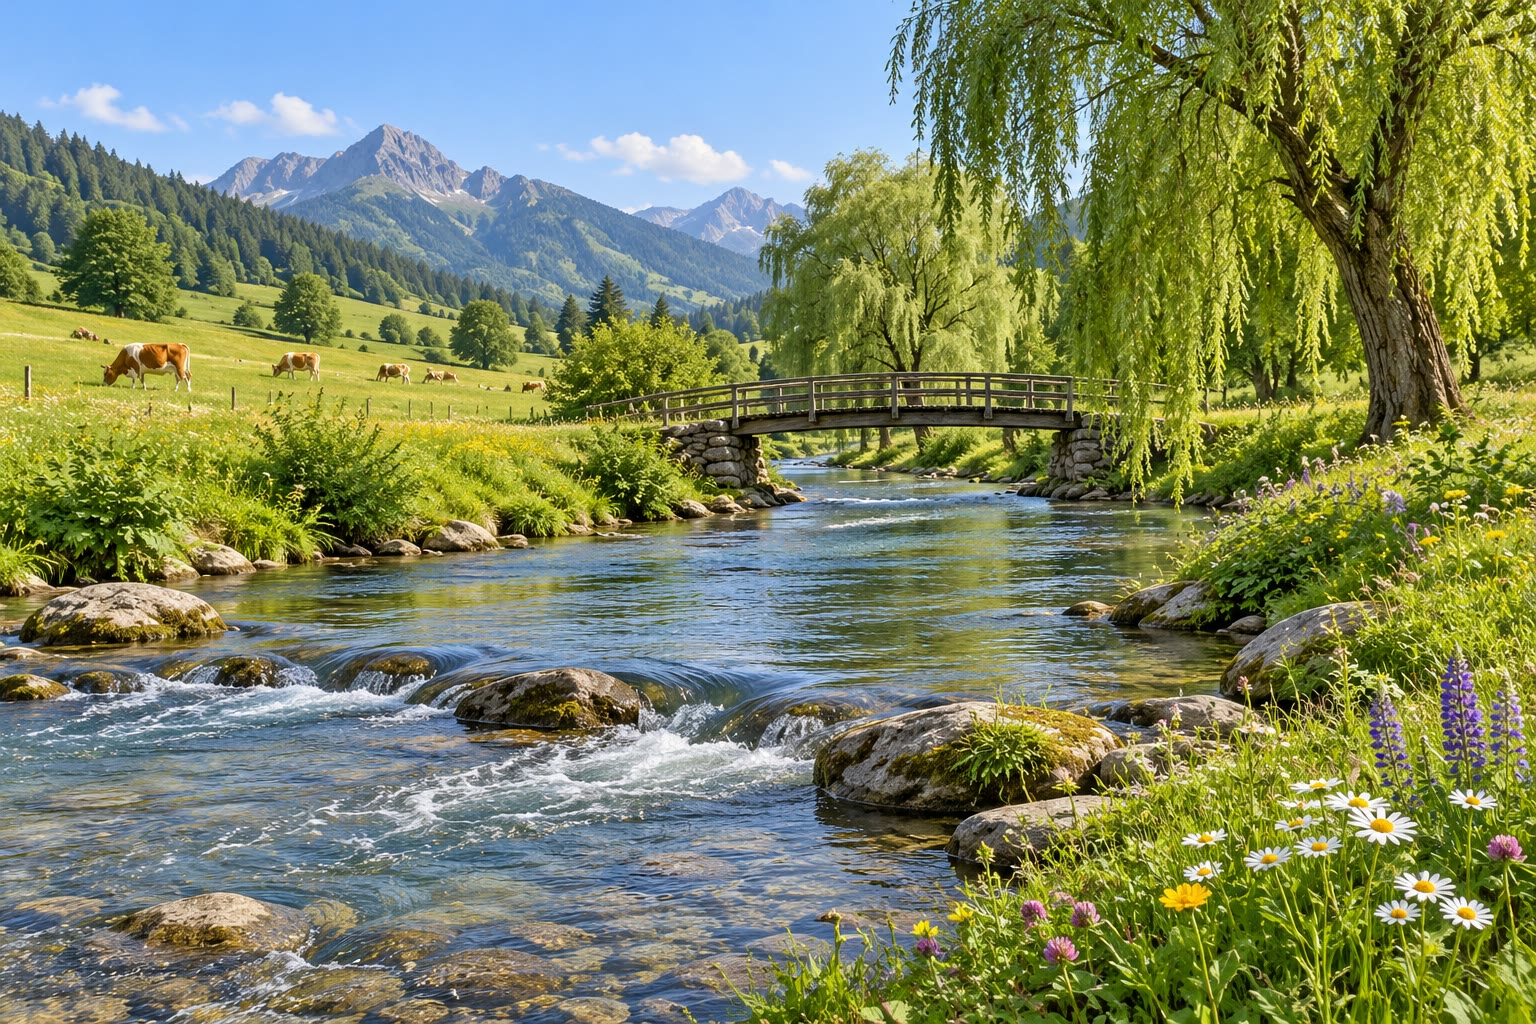
\includegraphics[width=\linewidth]{images/book1/ai/g2-river-meadow.jpg}

{\small \omterm{def:g2:water-on-earth:salt-fresh}{Água doce}: um \omterm{def:g1:landscapes-around-us:water}{rio}.}
\end{minipage}\hfill
\begin{minipage}[b]{0.49\linewidth}\centering
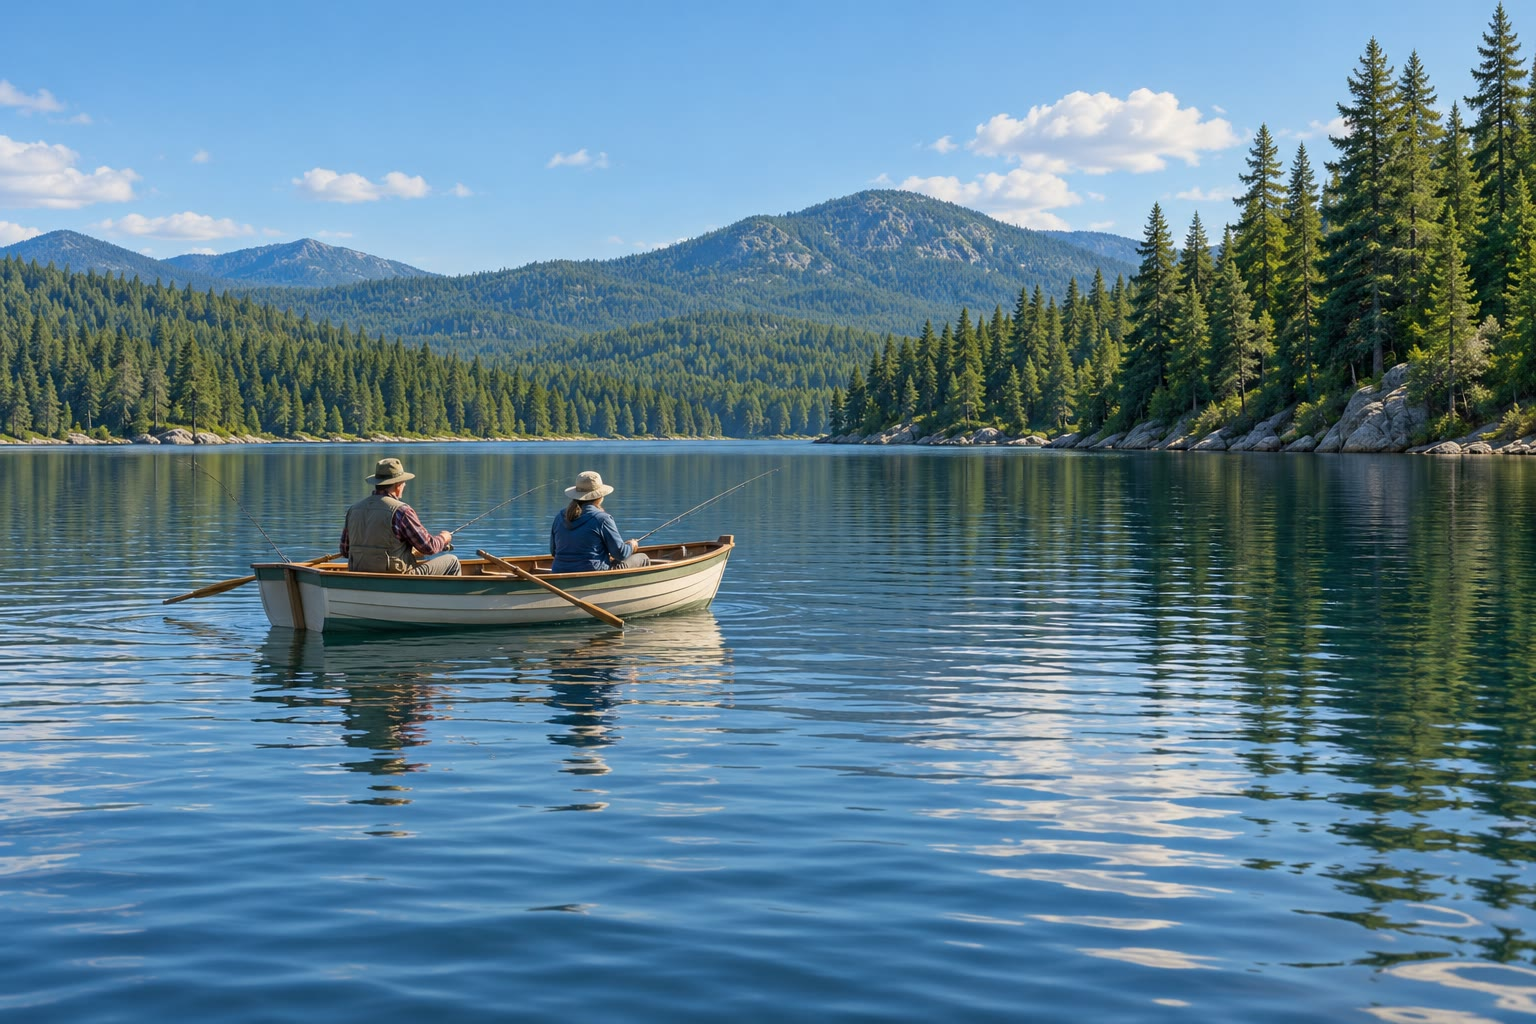
\includegraphics[width=\linewidth]{images/book1/ai/g2-lake-boat.jpg}

{\small \omterm{def:g2:water-on-earth:salt-fresh}{Água doce}: um \omterm{def:g1:landscapes-around-us:water}{lago}.}
\end{minipage}
\end{omfigure}

\begin{remark}[Não podemos beber água do mar]\label{rem:g2:water-on-earth:drink}
As pessoas e os animais terrestres não podem beber água do \omterm{def:g2:water-on-earth:ocean}{mar}: ela tem
sal demais, e bebê-la faz o corpo perder água em vez de ganhar. Os
marinheiros em \omterm{def:g2:water-on-earth:ocean}{alto-mar}, cercados de água por todos os lados, sempre
precisaram levar a sua \omterm{def:g2:water-on-earth:salt-fresh}{água doce} com eles.
\end{remark}

\section{Onde está toda a água?}

A \omterm{def:g2:water-on-earth:salt-fresh}{água doce} não está só nos \omterm{def:g1:landscapes-around-us:water}{rios} e nos \omterm{def:g1:landscapes-around-us:water}{lagos}. Muita \omterm{def:g2:water-on-earth:salt-fresh}{água doce} está
congelada: no grande gelo branco da Antártida e da Groenlândia, e no alto
das \omterm{def:g1:landscapes-around-us:landform}{montanhas}. E muita está escondida sob os nossos pés, no chão, onde
preenche os espacinhos entre os grãos de areia e as rachaduras da rocha.

\begin{omfigure}
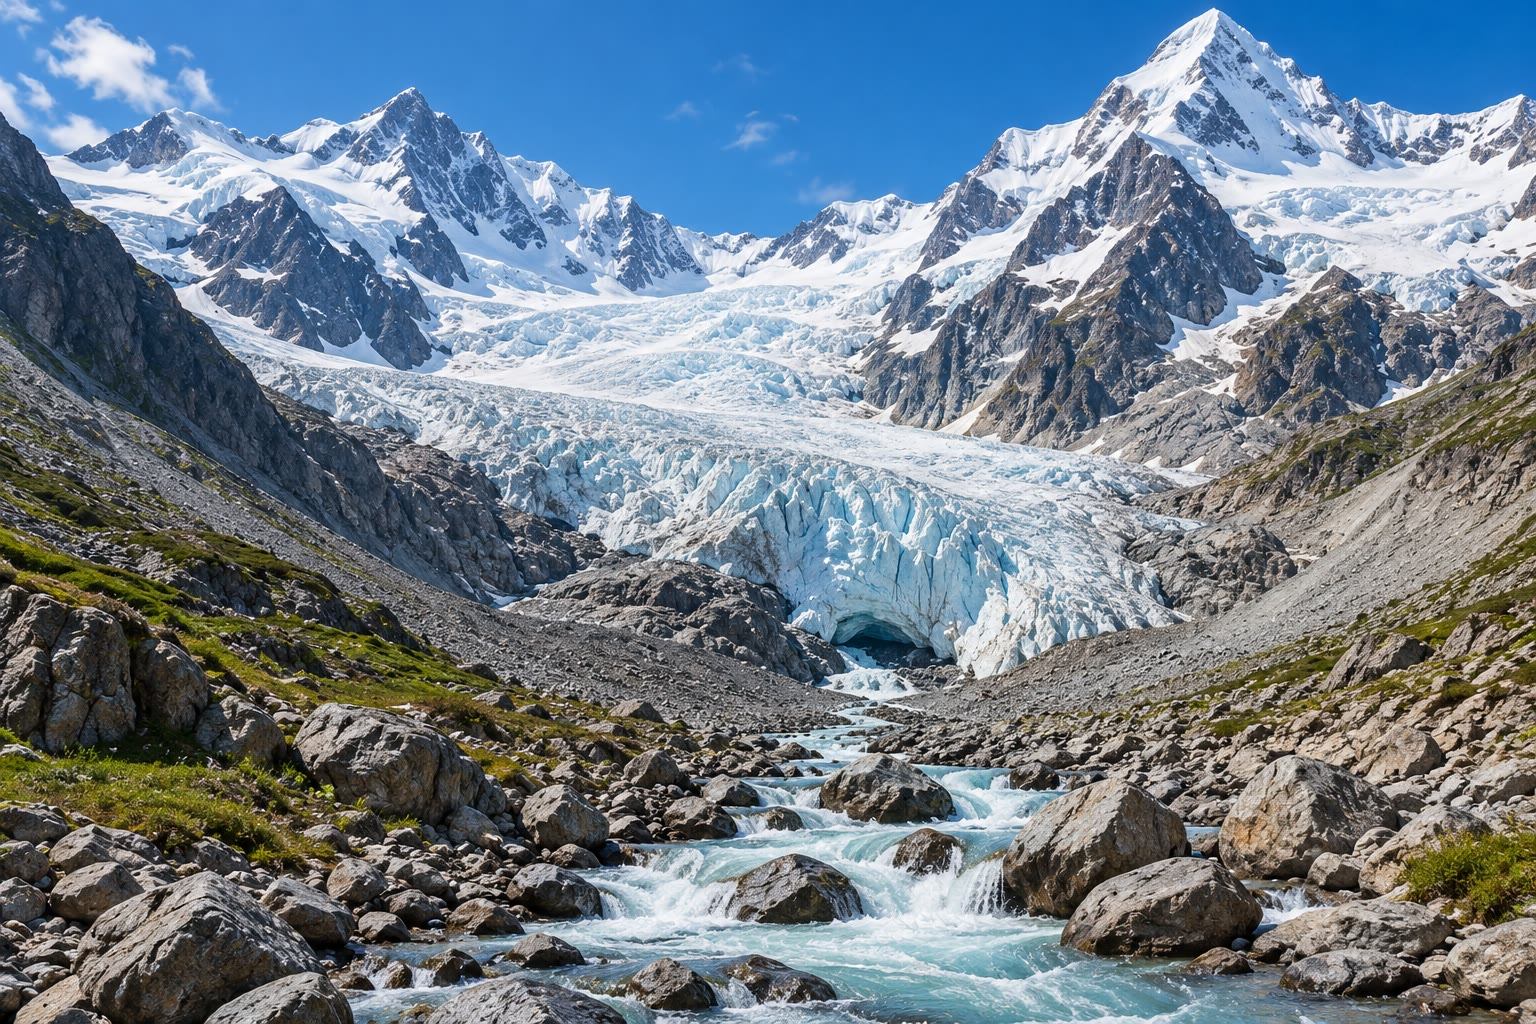
\includegraphics[width=0.62\linewidth]{images/book1/ai/g2-snowy-mountains.jpg}

{\small As \omterm{def:g1:landscapes-around-us:landform}{montanhas} altas guardam \omterm{def:g2:water-on-earth:salt-fresh}{água doce} em forma de neve e gelo o ano
inteiro. No verão, uma parte derrete e alimenta os riachos.}
\end{omfigure}

Imagine que pudéssemos despejar toda a água da Terra em 100 baldes do
mesmo tamanho. Quantos baldes cada tipo de água encheria?

\begin{omfigure}
\begin{tikzpicture}
  \begin{axis}[hide axis, width=7.2cm, height=7.2cm, xmin=-0.5, xmax=9.5,
      ymin=-0.5, ymax=9.5, axis equal image, scale only axis, clip=false]
    \addplot[scatter, only marks, mark=*, mark size=8pt,
      scatter/classes={0={fill=omSea!80!blue, draw=black!40},
                       1={fill=white, draw=black!60},
                       2={fill=brown!55, draw=black!40}},
      point meta=explicit symbolic]
      table[x=col, y=row, meta=kind] {figdata/out/grade-2-water_shares.dat};
  \end{axis}
  \begin{scope}[shift={(7.9,5.6)}, font=\small]
    \fill[omSea!80!blue, draw=black!40] (0,0) circle (0.2);
    \node[anchor=west] at (0.35,0) {água salgada dos oceanos: 96 baldes};
    \fill[white, draw=black!60] (0,-0.7) circle (0.2);
    \node[anchor=west] at (0.35,-0.7) {gelo e neve: 2 baldes};
    \fill[brown!55, draw=black!40] (0,-1.4) circle (0.2);
    \node[anchor=west] at (0.35,-1.4) {água embaixo da terra: 2 baldes};
  \end{scope}
\end{tikzpicture}

{\small Toda a água da Terra em 100 baldes. Os \omterm{def:g1:landscapes-around-us:water}{rios}, os \omterm{def:g1:landscapes-around-us:water}{lagos}, as nuvens e
a água de todos os seres vivos, juntos, não encheriam nem um balde.
Números do Serviço Geológico dos Estados Unidos (USGS).}
\label{fig:g2:water-on-earth:buckets}
\end{omfigure}
% ledger: wss:water-shares (rounded to 100 buckets in figdata/grade-2/water_shares.py)

\begin{proposition}[A maior parte da água da Terra é salgada]\label{prop:g2:water-on-earth:most-salty}
% ledger: wss:water-shares
De 100 baldes com toda a água da Terra, 96 são a \omterm{def:g2:water-on-earth:salt-fresh}{água salgada} dos
\omterm{def:g2:water-on-earth:ocean}{oceanos}. A \omterm{def:g2:water-on-earth:salt-fresh}{água doce} que bebemos é só uma parte bem pequena de toda a
água: a maior parte dela está congelada no gelo ou escondida embaixo da terra.
\end{proposition}

\section{Para onde vai a chuva?}

Quando chove, a água não fica onde cai. Observe o pátio da escola depois
de uma pancada de chuva: uma parte da água escorre pelo chão até as
sarjetas, outra parte se infiltra na terra dos canteiros, e as poças
somem aos poucos quando o sol volta.

\begin{omfigure}
\begin{tikzpicture}[x=1cm, y=1cm, font=\small]
  % sky, sea, land
  \fill[ocBlue!6] (0,0) rectangle (12,5.6);
  \fill[omSea] (8.6,0) rectangle (12,0.9);
  \fill[green!30!omLithAlluv] (0,0) -- (0,2.4) .. controls (2,2.6) and (3,2.0) .. (4.5,1.6)
     .. controls (6,1.2) and (7.5,1.0) .. (8.6,0.9) -- (8.6,0) -- cycle;
  % ground below the surface
  \fill[brown!25] (0,0) rectangle (8.6,0.6);
  % river
  \draw[omSea!70!blue, line width=2.4pt] (1.6,2.45) .. controls (3.5,2.0) and (6,1.15) .. (8.6,0.95);
  % cloud and rain
  \pic at (2.2,4.0) {puffycloud};
  \foreach \x in {1.4,1.8,2.2,2.6,3.0}
    \draw[omWxRain, line width=0.8pt] (\x,3.7) -- (\x-0.15,3.1);
  \pic at (9.6,4.3) {puffycloud};
  % arrows
  \draw[omWxRain, line width=1.1pt, -{Stealth[length=2.5mm]}] (3.3,2.15) -- (3.3,0.6);
  \node[anchor=west, align=left, font=\scriptsize] at (3.4,1.0) {uma parte\\entra no chão};
  \draw[omWxRain, line width=1.1pt, -{Stealth[length=2.5mm]}] (5.4,1.55) -- (7.6,1.15);
  \node[align=center, font=\scriptsize] at (6.2,2.05) {uma parte vai para um rio,\\e o rio corre para o mar};
  \draw[black!50, line width=1.1pt, densely dashed, -{Stealth[length=2.5mm]}] (10.2,1.1) .. controls (10.4,2.4) and (10.1,3.2) .. (9.8,3.85);
  \node[align=left, anchor=west, font=\scriptsize] at (10.45,2.4) {a água\\evapora};
  \draw[black!50, line width=1.1pt, densely dashed, -{Stealth[length=2.5mm]}] (8.45,4.35) -- (3.6,4.3);
  \node[font=\scriptsize, above] at (6.0,4.35) {o vento leva as nuvens};
  \node[font=\scriptsize] at (10.4,0.45) {mar};
  \node[font=\scriptsize, anchor=west] at (0.2,3.25) {chuva};
\end{tikzpicture}

{\small Para onde vai a chuva. A água que sobe do \omterm{def:g2:water-on-earth:ocean}{mar} e da terra em forma
de vapor forma nuvens novas, e as nuvens trazem chuva nova.}
\label{fig:g2:water-on-earth:rain}
\end{omfigure}

\begin{method}[Seguir uma gota de chuva]\label{met:g2:water-on-earth:drop}
Para seguir uma gota de chuva, faça três perguntas, uma depois da outra:
\begin{enumerate}
  \item Onde ela cai: no \omterm{def:g2:water-on-earth:ocean}{mar}, num telhado, na terra, numa \omterm{def:g1:landscapes-around-us:landform}{montanha}?
  \item Ela entra no chão, escorre pela superfície ou congela e vira gelo?
  \item Para onde ela vai depois: para um \omterm{def:g1:landscapes-around-us:water}{rio}, um \omterm{def:g1:landscapes-around-us:water}{lago}, o \omterm{def:g2:water-on-earth:ocean}{mar}, o chão, ou
        de volta para o ar?
\end{enumerate}
No fim, toda gota volta para o \omterm{def:g2:water-on-earth:ocean}{mar} ou para o ar, e a viagem começa de
novo.
\end{method}

\begin{example}[Uma gota na montanha]\label{ex:g2:water-on-earth:mountain}
Uma gota de chuva cai como neve numa \omterm{def:g1:landscapes-around-us:landform}{montanha} alta, no inverno. Ela fica
lá, congelada, até os dias quentes do verão. Então derrete, desce por um
riacho da \omterm{def:g1:landscapes-around-us:landform}{montanha}, chega a um \omterm{def:g1:landscapes-around-us:water}{rio}, e o \omterm{def:g1:landscapes-around-us:water}{rio} a leva até o \omterm{def:g2:water-on-earth:ocean}{mar}. Num dia de
sol, a gota evapora do \omterm{def:g2:water-on-earth:ocean}{mar} e sobe para o ar, onde passa a fazer parte de
uma nuvem nova.
\end{example}

\section{Exercícios}

\begin{exercise}[$\star$]\label{exo:g2:water-on-earth:1}
\omterm{def:g2:water-on-earth:salt-fresh}{Água salgada} ou \omterm{def:g2:water-on-earth:salt-fresh}{água doce}? O \omterm{def:g2:water-on-earth:ocean}{mar}; um \omterm{def:g1:landscapes-around-us:water}{rio}; a chuva; um \omterm{def:g1:landscapes-around-us:water}{lago} nas
\omterm{def:g1:landscapes-around-us:landform}{montanhas}; um \omterm{def:g2:water-on-earth:ocean}{oceano}; o gelo de uma \omterm{def:g1:landscapes-around-us:landform}{montanha}.
\end{exercise}

\begin{exercise}[$\star$]\label{exo:g2:water-on-earth:2}
Por que chamamos a Terra de ``planeta azul''?
\end{exercise}

\begin{exercise}[$\star$]\label{exo:g2:water-on-earth:3}
Na grade de 100 quadrados, 71 quadrados são azuis. Quantos quadrados são
de terra?
\end{exercise}

\begin{exercise}[$\star$]\label{exo:g2:water-on-earth:4}
O que é maior: um \omterm{def:g2:water-on-earth:ocean}{oceano} ou um \omterm{def:g2:water-on-earth:ocean}{mar}?
\end{exercise}

\begin{exercise}[$\star$]\label{exo:g2:water-on-earth:5}
Um marinheiro no meio do \omterm{def:g2:water-on-earth:ocean}{oceano} pode beber a água em volta do barco? Por
quê?
\end{exercise}

\begin{exercise}[$\star$]\label{exo:g2:water-on-earth:6}
Cite três lugares onde há \omterm{def:g2:water-on-earth:salt-fresh}{água doce}.
\end{exercise}

\begin{exercise}[$\star\star$]\label{exo:g2:water-on-earth:7}
No desenho dos 100 baldes, quantos baldes são de \omterm{def:g2:water-on-earth:salt-fresh}{água salgada}? Quantos
são de \omterm{def:g2:water-on-earth:salt-fresh}{água doce} (o gelo e a água embaixo da terra, juntos)?
\end{exercise}

\begin{exercise}[$\star\star$]\label{exo:g2:water-on-earth:8}
Coloque em ordem, do que guarda mais água para o que guarda menos: os
\omterm{def:g1:landscapes-around-us:water}{rios}; os \omterm{def:g2:water-on-earth:ocean}{oceanos}; o gelo e a neve.
\end{exercise}

\begin{exercise}[$\star\star$]\label{exo:g2:water-on-earth:9}
Chove numa plantação. Diga duas coisas que podem acontecer com a água.
\end{exercise}

\begin{exercise}[$\star\star$]\label{exo:g2:water-on-earth:10}
Uma panela com água do \omterm{def:g2:water-on-earth:ocean}{mar} fica no sol por muitos dias, até a água acabar.
O que sobra no fundo da panela? Para onde foi a água?
\end{exercise}

\begin{exercise}[$\star\star$]\label{exo:g2:water-on-earth:11}
Conte a viagem de uma gota de chuva que cai no telhado da escola, até ela
voltar a fazer parte de uma nuvem.
\end{exercise}
